\chapter{Considerações Finais}
\label{chapter:Consideracoes_Finais}

 Este documento completa a primeira etapa deste trabalho, onde foram apresentados os principais pontos pontos quanto ao tema proposto. Esta visão, em um contexto mais amplo, compreende aspectos relacionados a redes sociais e reutilização de software e apresenta a ideia geral de desenvolvimento de um \textit{framework}. Esse suporte procurará auxiliar na criação de redes sociais, oferecendo recursos gerais de relacionamento entre pessoas em uma rede virtual, bem como recursos específicos de rotas e agendas. A partir desses recursos, um desenvolvedor poderá usar este \textit{framework} usufruindo do suporte sem se preocupar, idealmente, com a lógica por trás de sua implementação.

 Em um contexto mais técnico, foram discutidas também algumas formas para desenvolver o que se propõe. Entre esses aspectos, foram apresentados pontos como teoria dos grafos, algoritmos relacionados e padrões de projeto.

Durante a construção deste documento, alguns passos foram seguidos buscando apresentar o tema e aspectos relacionados. Inicialmente, foi desenvolvida uma contextualização que traz o tema proposto de uma forma geral e apresenta ao leitor os objetivos deste trabalho. Logo após, foi feito um levantamento bibliográfico com o objetivo de buscar uma melhor adequação ao tema proposto. Esse passo colaborou com a elaboração do capítulo de ~\nameref{chapter:Referencial_Teorico}, onde estão presentes todos os temas pertinentes a esse trabalho, levantados até o momento. Foi feito também um levantamento das tecnologias e ferramentas que serão usadas durante este trabalho, as quais estão documentadas no capítulo de ~\nameref{chapter:Suporte_Tecnologico}. No capítulo de ~\nameref{chapter:Metodologia}, foram definidas as metodologias de pesquisa e de desenvolvimento. Por fim, concretizou-se a ~\nameref{chapter:Proposta} deste trabalho apresentando-a de uma forma mais completa e discorrendo sobre os principais pontos de forma mais técnica. Nessa etapa, também foi desenvolvida uma aplicação que serviu como prova de conceito para aprofundar os conhecimentos quanto às necessidades e dificuldades relacionadas à proposta, ou seja, ao desenvolvimento do \textit{framework} bem como de duas instanciações: uma voltada para o domínio de rotas e outra voltada para o domínio de agendas.

A tabela \ref{status atividades} apresenta os status das atividades que estão previstas no cronograma deste trabalho.

\newpage

\begin{table}[h]
\centering
\caption{Status das atividades previstas no cronograma}
\label{status atividades}
\begin{tabular}{|l|c|}
\hline
                                       & Status   \\ \hline
Elaborar Proposta Inicial              & Completa \\ \hline
Definir Escopo                         & Completa \\ \hline
Realizar Levantamento Bibliográfico    & Completa \\ \hline
Definir Metodologia de Desenvolvimento & Completa \\ \hline
Definir Suporte Tecnológico            & Completa \\ \hline
Estabelecer Proposta                   & Completa \\ \hline
Desenvolver Prova de Conceito          & Completa \\ \hline
Apresentar TCC1                        & A Fazer  \\ \hline
Refinar TCC1                           & A Fazer  \\ \hline
Desenvolver o Framework                & A Fazer  \\ \hline
Desenvolver a Rede Social              & A Fazer  \\ \hline
Coletar e Avaliar Resultados           & A Fazer  \\ \hline
Apresentar TCC2                        & A Fazer  \\ \hline
Refinar TCC2                           & A Fazer  \\ \hline
\end{tabular}
\end{table}

Pode-se então ter uma ideia da quantidade do trabalho completo falta ser realizado, de acordo com o gráfico apresentado na figura \ref{status projeto}. Esses valores levam em consideração a complexidade atribuída às atividades apresentadas.

\begin{figure}[!h]
	\centering
	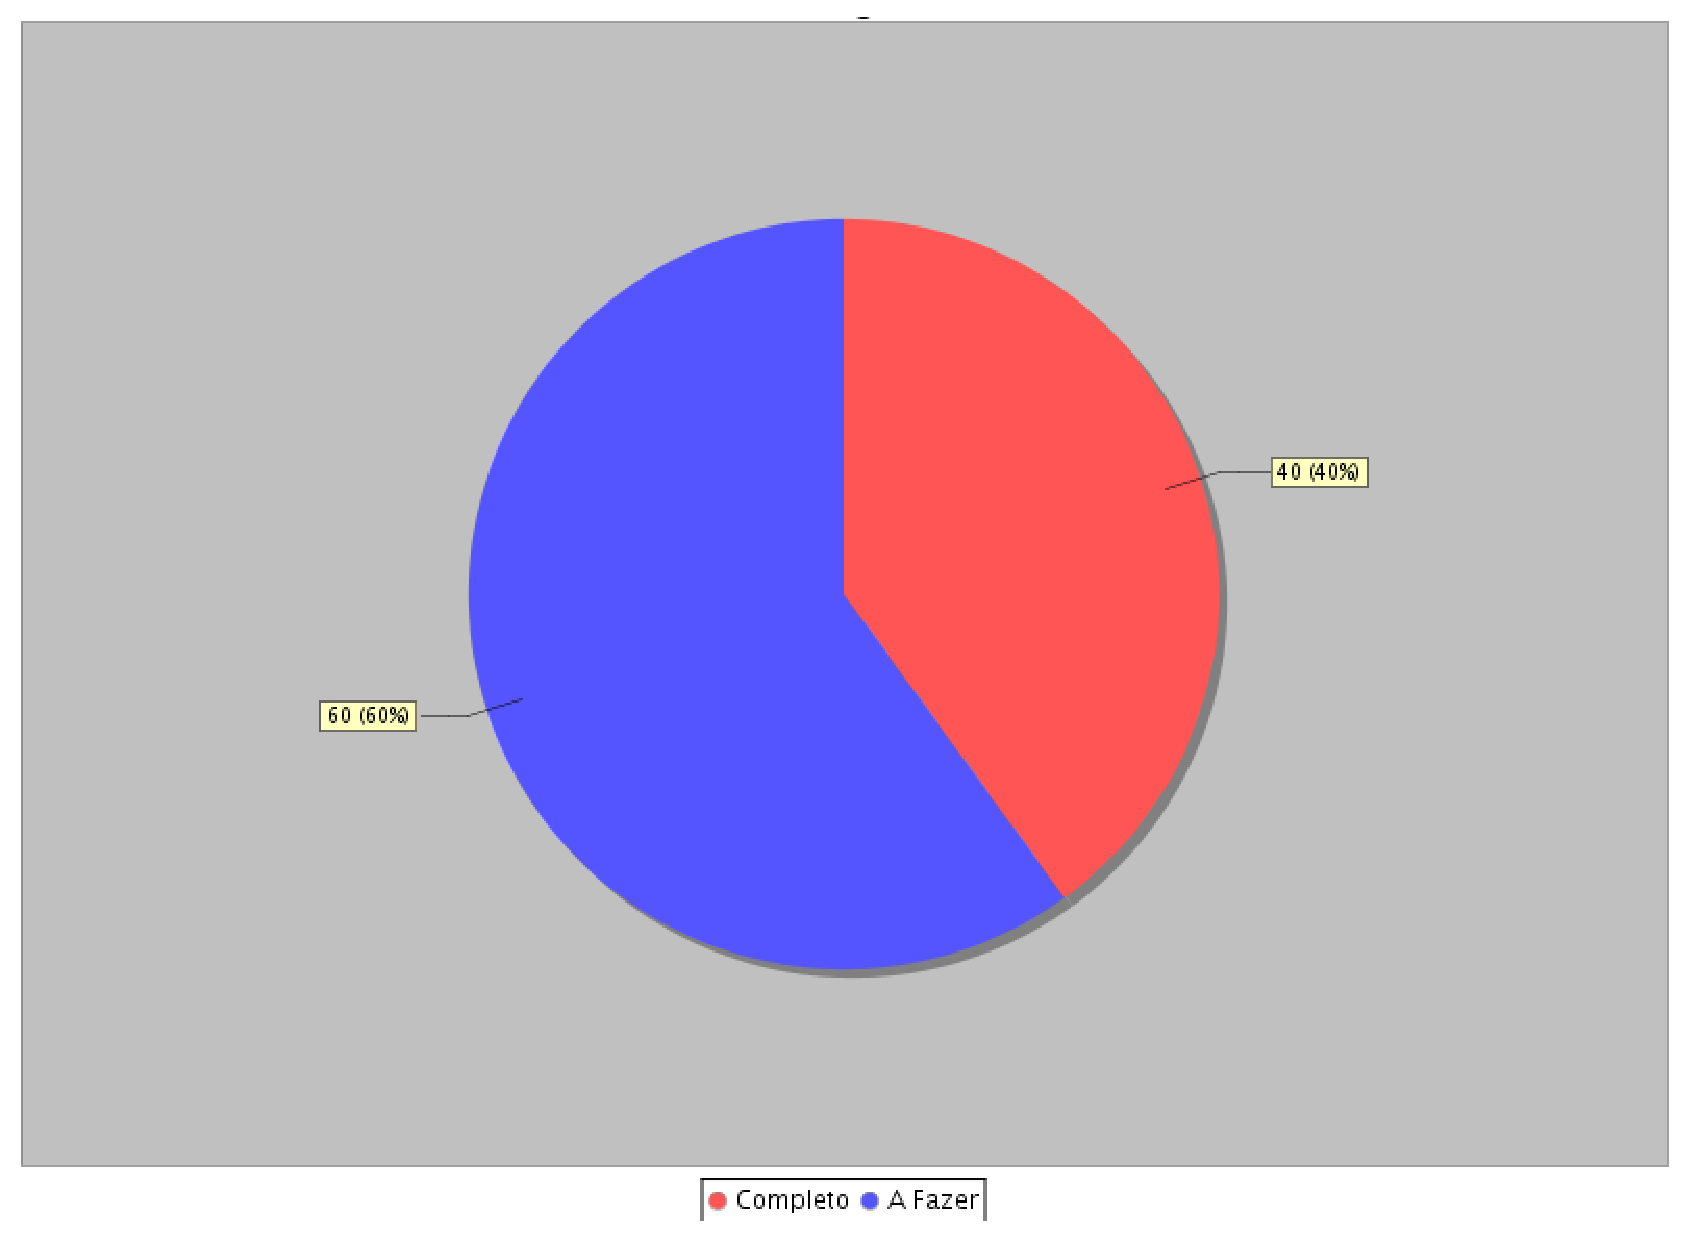
\includegraphics[scale=0.5]{figuras/capitulo6/status_projeto.eps}
	\caption{Status do projeto}
	\label{status projeto}
\end{figure}

Pode-se considerar que a primeira etapa desta trabalho está completa. A próxima etapa levará em consideração tudo que foi investigado, desenvolvido e contemplado até o momento. Posteriormente, serão inicializadas as etapas que compreendem maior esforço de desenvolvimento. Na primeira etapa de desenvolvimento, os requisitos detalhados do \textit{framework} serão levantados, o que conduzirá à especificação do \textit{backlog} do produto. Esse, por sua vez, servirá de base para a criação e a priorização das \textit{sprints}, onde de fato o código do \textit{framework} será desenvolvido. A segunda etapa compreende o desenvolvimento de uma aplicação que instanciará o \textit{framework} proposto. Por fim, os resultados serão coletados e apresentados para finalização de todo o trabalho.
